\sys is a new programming and execution model for intermittent computing on energy-harvesting devices. \sys addresses the challenges outlined in Section~\ref{sec:background} to make task-based intermittent programs {\em programmable} and {\em efficient}. \sys accomplishes this goal with a constellation of a new programming model and run time software system support, that supports dynamically adaptive task-based execution. Figure~\ref{fig:system_overview} shows an overview of \sys.

\begin{figure}
	\centering
	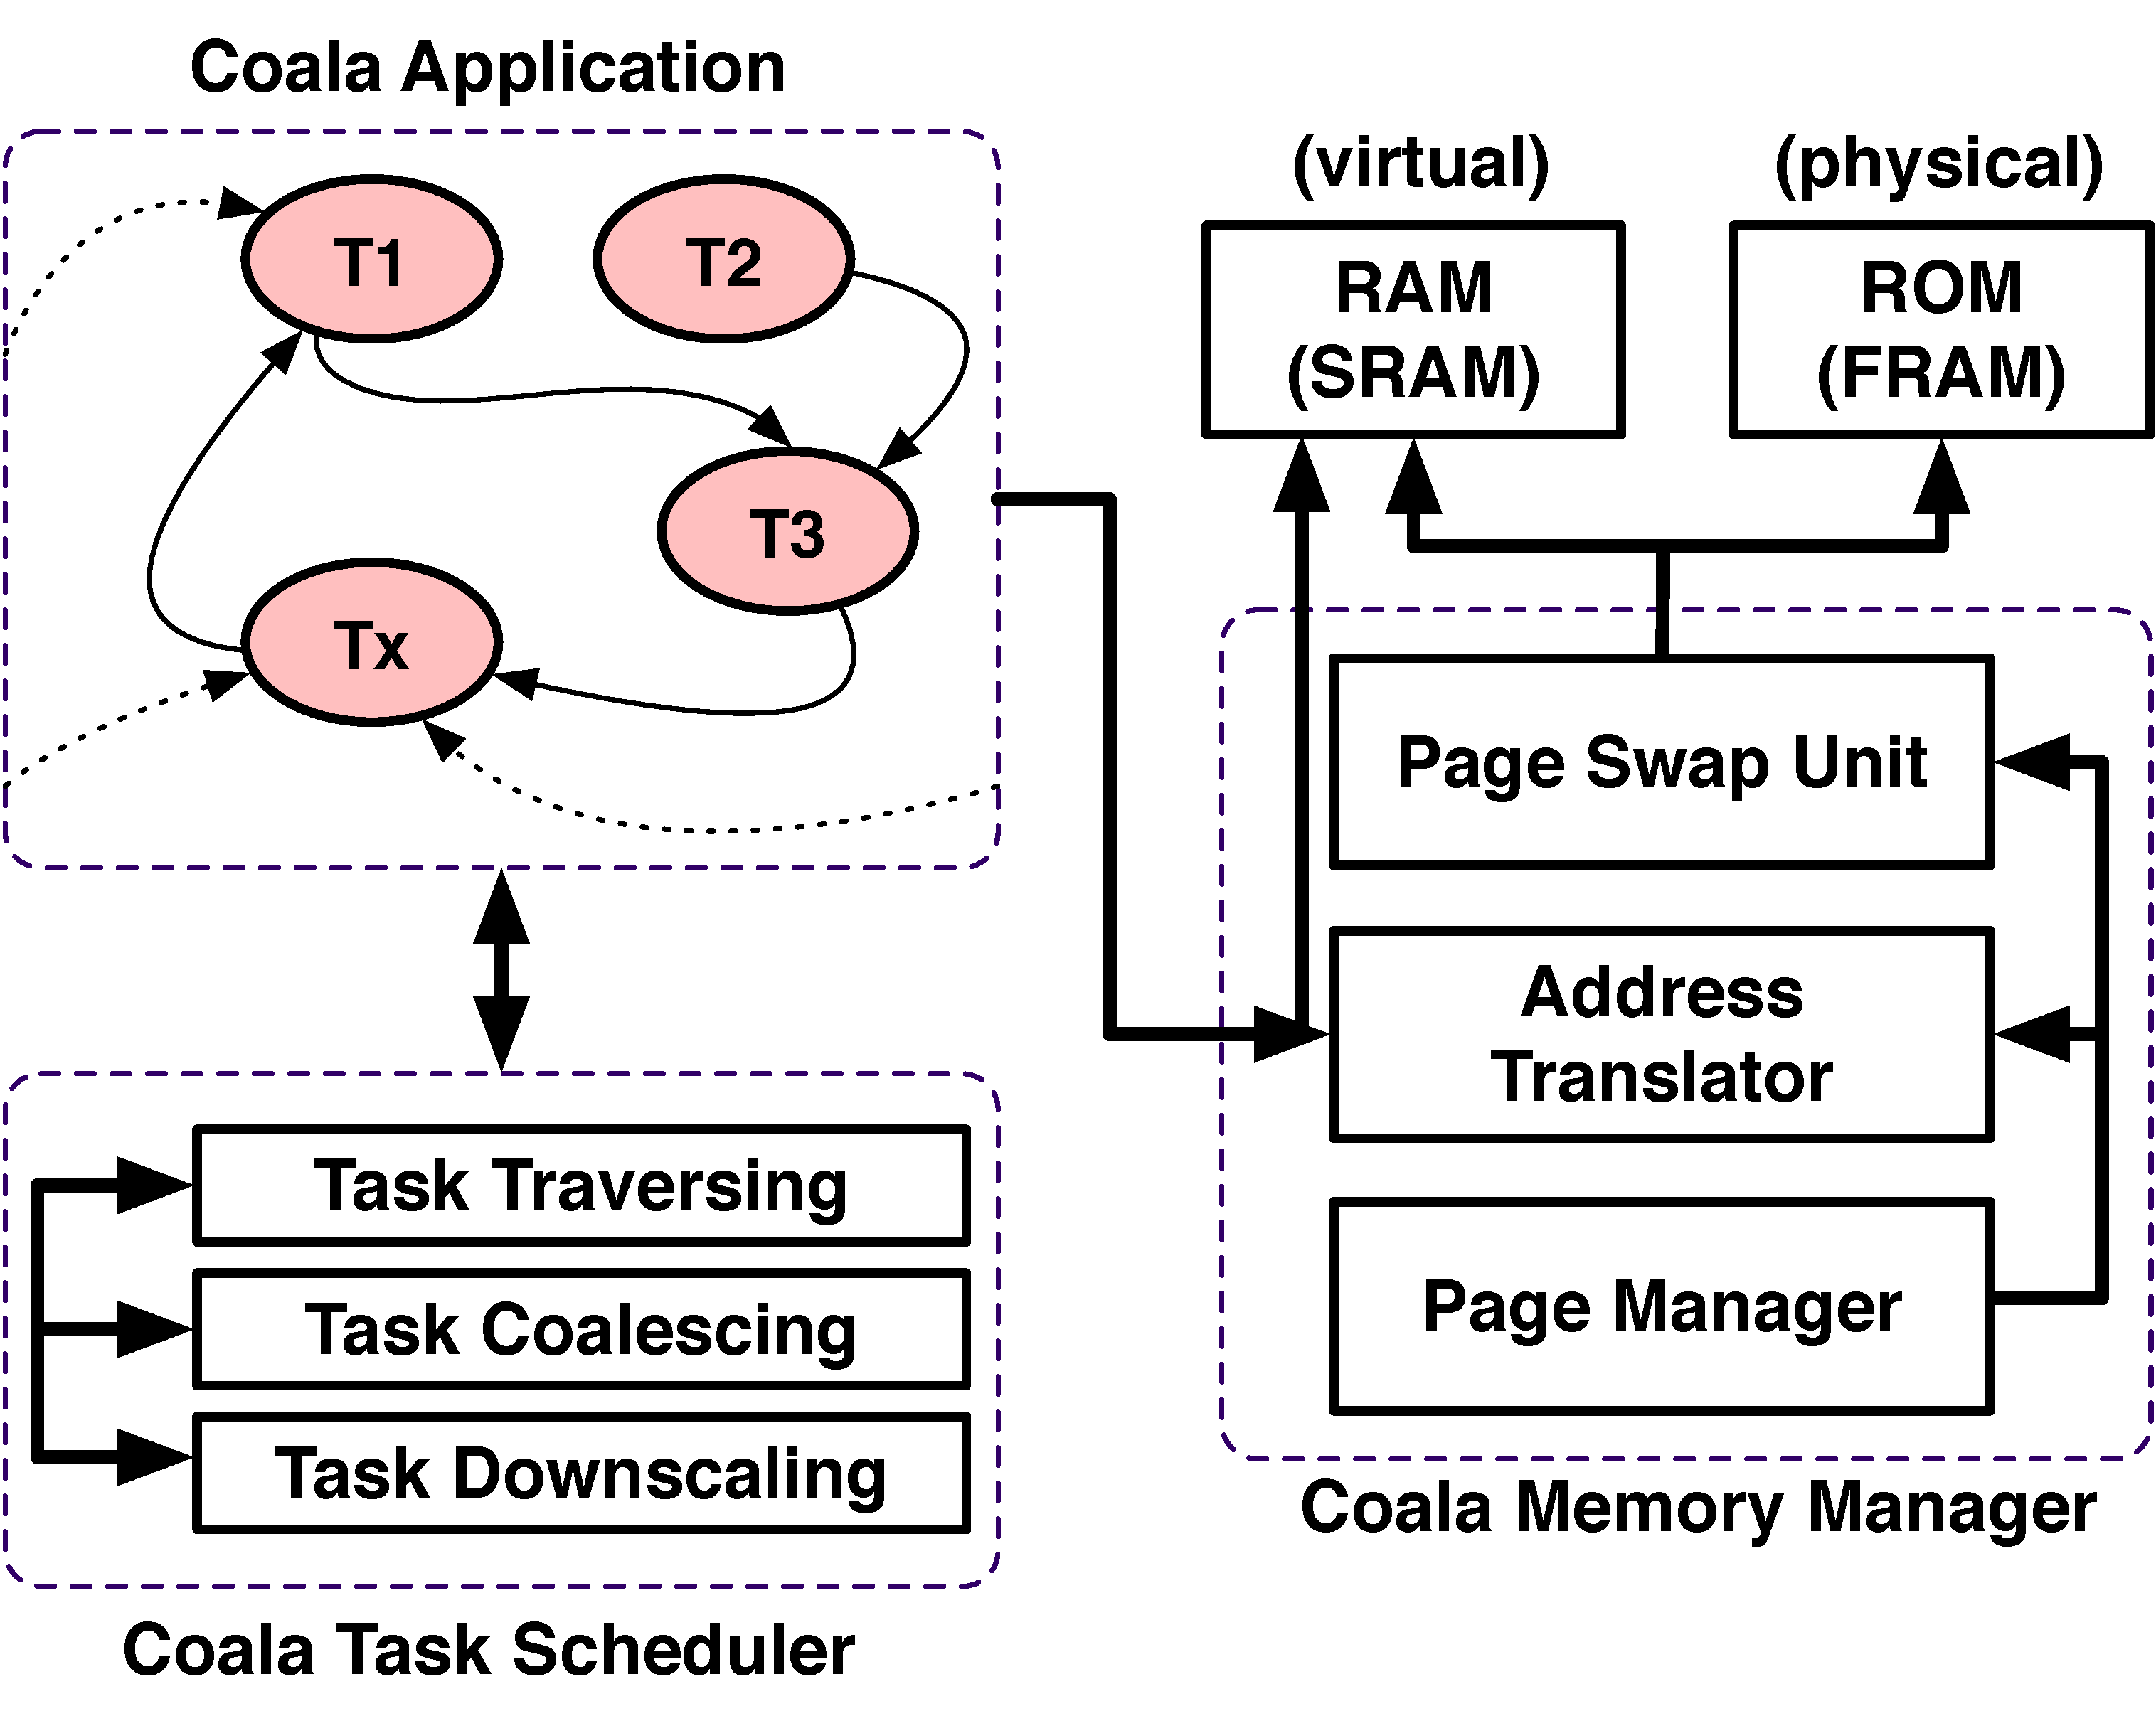
\includegraphics[width=\columnwidth]{figures/graffle/overview.pdf}
	\caption{\sys top-level view. \textcolor{red}{redraw the figure: remove compiler, add task downscaling}}
	\label{fig:system_overview}
\end{figure}

\textbf{\sys Programming and Execution Model.}  To use \sys, a programmer first writes plain, imperative C code. The programmer
then must decompose the program into tasks. To manually decompose a program into tasks, the programmer designates a set of functions as tasks, sequences control-flow between these tasks, and annotates memory accesses that manipulate data shared by multiple tasks. 

%\sys's programming interface, listed in Table~\ref{tab:viper_syntax}, consists of primitives for defining tasks~\cite{chain,alpaca} and accessors for protected variables shared between tasks.
%
%As in prior task-based intermittent programming models~\cite{chain,alpaca}, tasks are functions that are not allowed to have any direct callers but receive control via explicit {\tt next\_task} statements only. The programmer identifies each task by adding the {\tt task} keyword to the function's declaration and designates one task as the {\em origin} task at which execution begins. After a power failure, \sys restarts the last partially executed task.
%
%A \sys program manipulates {\em protected} state---accessed by more than one task---using the \emph{read variable} ({\tt RVAR}) and \emph{write variable} ({\tt WVAR}) operations. These operations convey to \sys that the referenced data are task-shared, meaning that they must be buffered in volatile memory and committed when the executing task ends.
%
%Commit is a key overhead associated with task-based operation and \sys's coalescing strategy (described in Section~\ref{sec:coalescing} avoids commit when a task ends by continuing to buffer task-shared variables for multiple coalesced tasks, and committing only when all tasks complete.

%\begin{table}
%	\centering
%	\footnotesize
%	\begin{tabular}{|c|c|}
%		\hline
%		\textbf{Keyword} & \textbf{Description} \\
%		\hline\hline
%		\texttt{task foo() \{...\}} & Task definition\\
%		\texttt{origin task foo() \{...\}} & Origin task definition\\
%		\texttt{next\_task(t)} & Transition to task \texttt{t}\\
%		\texttt{u = RVAR(v)} & Read protected variable \texttt{v} into \texttt{u}\\
%		\texttt{WVAR(v, u)} & Write \texttt{u} to protected variable \texttt{v}\\
%		\hline
%	\end{tabular}
%	\caption{\sys's programming interface.}
%	\label{tab:viper_syntax}
%\end{table}

The programmer can decompose a program into tasks either {\em manually}. To do so manually,  requires reasoning similar to prior
task-based systems~\cite{chain,alpaca}.  
%
%A programmer may also opt to use compiler support to automatically decompose a program into tasks, leveraging recent work~\cite{cleancut,baghsorkhi_cgo_2018}.
%
%Without loss of generality, we assume throughout this work that the programmer manually decomposed the program into tasks; \sys's behavior with automatically decomposed code would be identical.

%Regardless of whether automatically or manually decomposed into tasks, the
%
The programmer compiles their task-based code, and links to the \sys runtime, producing a \sys-enabled binary. The \sys runtime implements \sys's task-based programming and execution model. The runtime system also includes \sys's novel {\em virtualizing memory manager} and its {\em task coalescing manager}, and {\em task downscaling manager}, both of which are essential to \sys's adaptive task-based execution.

\textbf{\sys Task Coalescing Manager.} \sys relies on its task coalescing manager to dynamically {\em coalesce} statically\hyp{}defined tasks to avoid inessential overheads associated with completing tasks. By default, tasks run in a sequence and each task commits its task-shared state as it completes.  The time and energy cost of a task's commit is unnecessary if the task and its successor both complete without a power failure. The key insight that \sys leverages is that the first task could have deferred its commit to the second task. {\em coalescing} tasks by deferring the first commit avoids the fixed cost of the first commit (task transitioning overheads). Coalescing also amortizes per-variable commit cost, committing each  location accessed by both tasks only after the second task, rather than once per task.

\textbf{\sys Task Downscaling Manager.} \textcolor{red}{to be written}
 
\textbf{\sys Virtual Memory Manager.}  \sys is able to efficiently coalesce tasks because of its efficient virtual memory manager, which is described in Section~\ref{sec:memory_virtualization}. \sys's memory manager paginates memory and ensures that data in a page remain consistent despite power interruptions. \sys allows a task to manipulate data in a volatile copy of a page only. Pages swap between volatile and non-volatile memory, depending on the capacity of the volatile memory and the program's access pattern. \sys tracks a task's memory accesses efficiently at page granularity (rather than using, e.g., costly word-granular tracking). When a task ends, each page it accessed commits from volatile memory (or from a non-volatile swap region for dirty pages) back to the non-volatile main memory. Pages efficiently, atomically commit using a two-phase commit procedure accelerated using hardware support for direct memory access (DMA).